%!TEX root = ../../main.tex
\section{킬을 묶는 시간과 거리의 경계}
\label{sec:eng-temporal}
\label{sec:eng-spatial}

킬을 교전으로 묶으려면 두 가지를 정해야 한다. 잇따른 킬을 얼마나 떨어진 시간까지 한 묶음으로 볼 것인가, 그리고 시간이 가까워도 지도에서 얼마나 떨어지면 다른 전투로 볼 것인가이다.

앞의 것이 시간 경계이다. 한 경기의 킬을 시간 순으로 훑으면서, 잇따른 두 킬의 간격이 시간 경계보다 짧으면 같은 묶음에 넣고 그보다 길면 거기서 묶음을 끊는다. 이 경계를 $G$라 쓴다. 남는 문제는 $G$를 얼마로 둘 것인가이다.

제 \ref{sec:rel-encounter} 절에서 보았듯 이전 연구는 두 값을 게임의 성질로 정했고 자료에서 얻은 근거를 남기지 않았다. 본 논문은 값을 고르는 대신 자료에서 읽는다. 잇따른 사건의 간격을 모으면 같은 묶음 안의 간격과 묶음 사이의 간격이 서로 다른 봉우리를 이루므로, 경계를 두 봉우리 사이의 가장 낮은 곳에 두는 것이다. 이 방법에는 선례가 있다. 활동 사이의 간격에서 세션의 경계를 읽는 연구 \cite{halfaker2015session,mehrzadi2012session}와 시공간의 최근접 거리에서 지진 군집을 가르는 연구 \cite{zaliapin2013clusters}가 같은 구조를 쓰고, 봉우리를 찾는 도구는 커널 밀도 추정이다 \cite{silverman1981multimodality}. 세션 연구에는 한 번 자료에서 얻은 값이 다시 추정되지 않은 채 관례로 굳은 예도 있다 \cite{mehrzadi2012session}. 그래서 본 논문은 추정을 한 번의 계산이 아니라 다시 돌릴 수 있는 절차로 두었다.

추정은 표본이 아니라 코퍼스 전체에서 한다. 세 패치의 경기 가운데 킬 사이의 간격이 하나 이상인 모든 경기, 곧 \numMatchesDef{} 경기의 간격 \numIntervalsDef{}개가 대상이다. 패치당 3{,}000 경기의 파일럿도 함께 두었는데, 파일럿에서는 패치별 값의 퍼짐이 더 컸고 전체 코퍼스에서 그 퍼짐이 줄었다. 파일럿에서 한 패치가 벗어나 보인 것은 표본의 잡음이었다.

그림 \ref{fig:kill-gap-kde}가 그렇게 그린 분포이다. 로그 척도에서 간격은 전투 안 \constGmodeIn{}초와 전투 사이 \constGmodeOut{}초에 봉우리를 갖고, 가장 낮은 곳은 \constGest{}초이다. 경기를 다시 뽑아 구한 95\% 구간은 \constGciLo{}--\constGciHi{}초인데, 각 반복이 간격의 일부만 쓰므로 코퍼스가 허용하는 것보다 넓다. 커널의 폭을 바꾸면 그 지점은 13.6--14.1초 사이를 움직인다. 검출기는 \constG{}초로 실행하였다.

%% figure 객체: fig:kill-gap-kde — 잇따른 킬 사이 간격의 커널 밀도와 시간 경계.
%% 원본 figures/kill_gap_kde.png. 저장소의 잠긴 경계 기록에서 곡선을 되살려 그린 것이며,
%% 되살린 봉우리·골·깊이가 기록값과 일치함이 확인되어 있다 (lock_match).
\begin{figure}[t]
  \centering
  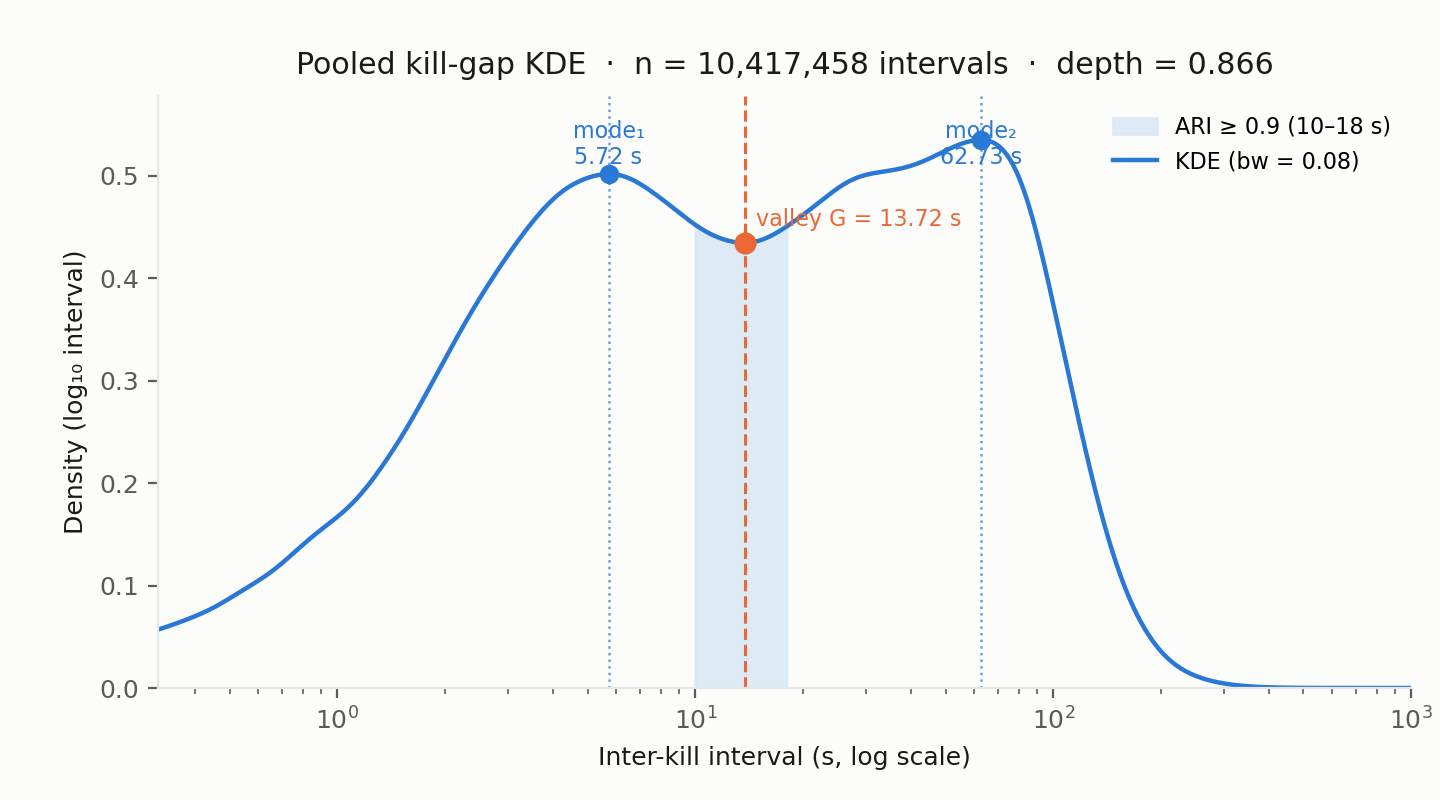
\includegraphics[width=\linewidth]{figures/kill_gap_kde.png}
  \caption{잇따른 킬 사이 간격의 분포와 시간 경계}
  \label{fig:kill-gap-kde}
\end{figure}


패치는 게임의 규칙을 바꾸므로 경계도 패치마다 다시 추정한다 \cite{chitayat2023beyond}. 세 패치는 각각 \constGpatchA{}, \constGpatchB{}, \constGpatchC{}초를 주며, 하나의 정의로 세 패치를 모두 덮을 수 있는지는 미리 정한 규칙으로 판정한다. 이 코퍼스에서는 하나로 충분하다는 판정이 나왔다. 그림 \ref{fig:boundary-per-patch}의 왼쪽이 패치별 시간 경계이고, 오른쪽은 뒤에서 정하는 거리 경계이다.

%% figure 객체: fig:boundary-per-patch — 패치별 시간·거리 경계와 합동 값.
%% 원본 figures/boundary_per_patch.png (저장소 경계 파이프라인의 산출물).
\begin{figure}[!t]
  \centering
  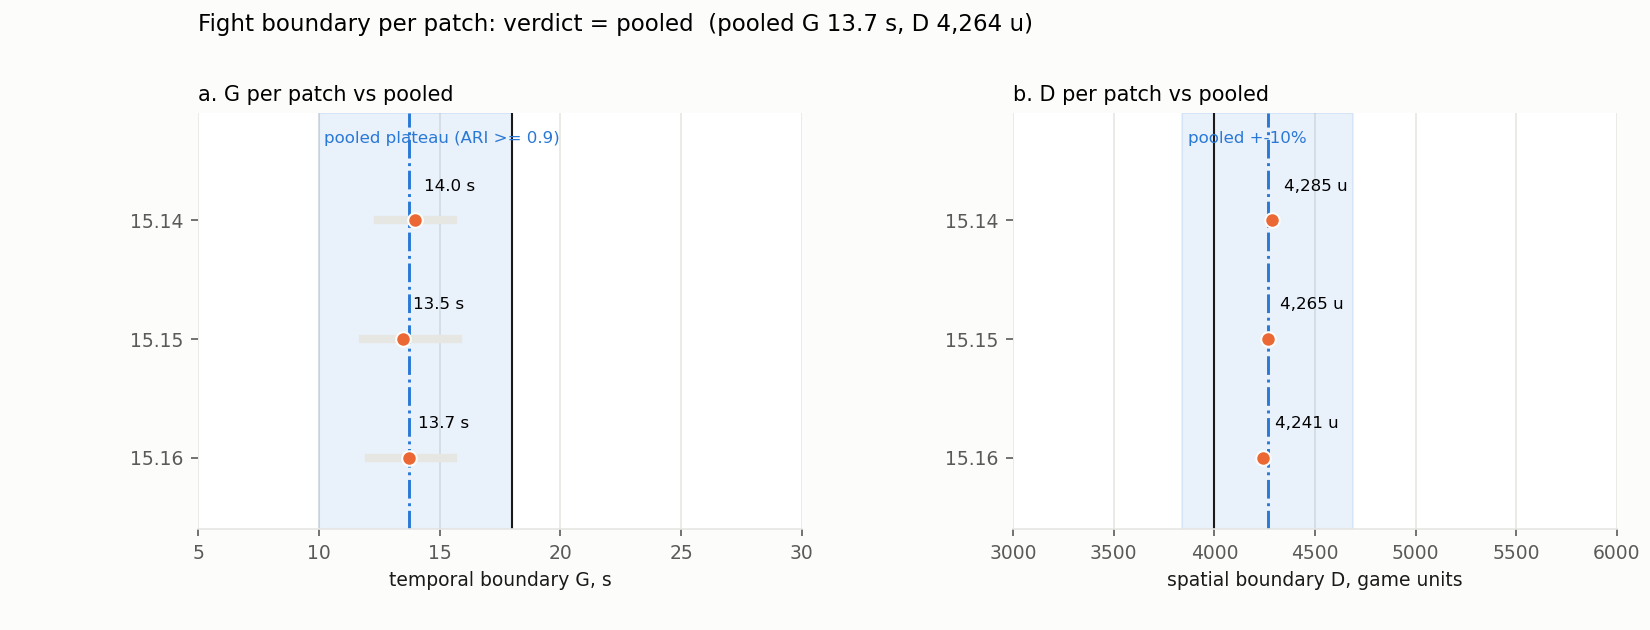
\includegraphics[width=\linewidth]{figures/boundary_per_patch.png}
  \caption{패치별 시간 경계와 거리 경계}
  \label{fig:boundary-per-patch}
\end{figure}


경계를 조금 옮겨도 묶음은 거의 같다. 두 분할이 같은 킬을 얼마나 비슷하게 묶는지는 조정 랜드 지수로 재며, 같으면 1이고 우연 수준이면 0에 가깝다 \cite{hubert1985comparing}. \ariPlateauLo{}--\ariPlateauHi{}초의 모든 시험값에서 이 지수는 0.9를 넘는다. 상수를 값 하나가 아니라 이렇게 넓은 구간에서 고르는 것은 안정성을 기준으로 삼는 군집 선택의 방식을 따른 것이다 \cite{campello2013hdbscan}. Baek과 Kwon \cite{baek2026killconditioned}이 게임의 성질로 정한 \cogGap{}초도 자료에서 얻은 값과 거의 같은 묶음을 만든다(\ariVsEighteen{}). 달라지는 것은 묶음이 아니라 상수의 근거이다.

시간이 가까운 킬이라도 다른 전투일 수 있다. 두 라인에서 동시에 벌어지는 전투가 그 예이다. 그래서 한 묶음 안의 어떤 두 킬도 거리 경계 $D$보다 멀지 않도록 나눈다. 킬을 시간 순으로 보며, 이미 있는 묶음 가운데 구성원 모두가 $D$ 안에 있는 첫 묶음에 넣고, 없으면 새 묶음을 만든다.

$D$는 시간 규칙이 쓰지 않는 신호로 추정한다. 잇따른 두 킬이 같은 챔피언을 킬러나 희생자나 어시스트로 공유하는지이다. 한 챔피언이 동시에 두 곳에 있을 수 없으므로, 거리에 따른 공유율은 같은 전투가 어디서 끝나는지를 보여 준다. 경계는 그 비율이 0.5로 떨어지는 거리에 둔다. 시간 경계 안의 연속 쌍 \numPairsDef{}개에서 그 거리는 \constDest{} 단위이고, 경기를 다시 뽑아 구한 95\% 구간은 \constDciLo{}--\constDciHi{} 단위이다. 규칙이 잇는 쌍은 \shareLinkedPairs{}\%가 챔피언을 공유하고, 시간은 가깝지만 규칙이 나누는 쌍은 \shareSeparatedPairs{}\%만 공유한다. 검출기는 \constD{} 단위로 실행하였다.

이 값도 코퍼스 전체에서 얻었다. 파일럿에서 훨씬 넓었던 구간이 전체 코퍼스에서 좁아졌고, 파일럿이 풀지 못한 라인 방향과 가로 방향의 차이도 전체 코퍼스에서 드러났다. 다만 이 구간은 좁게 읽지 않는다. 공유율을 거리 구간별로 계산한 뒤 두 구간 사이를 직선으로 이어 얻은 값이므로, 구간이 재는 것은 표본의 변동뿐이고 직선이라는 가정의 오차는 들어 있지 않다. 해상도는 구간 간격인 750 단위 수준이다. 경계는 라인 방향이 가로 방향의 1.5--1.6배로 방향에 따라 다르지만, 타원으로 바꾸어도 다시 분류되는 쌍은 0.16\%에 그쳐 원형을 유지하였다. 세 패치의 값은 \constDpatchA{}, \constDpatchB{}, \constDpatchC{} 단위로 서로 10\% 안에 있다(그림 \ref{fig:boundary-per-patch}의 오른쪽).
